Although the multigrid method is most useful for 2D and 3D problems,
let us learn how to use it with a simple 1-D problem.
NOTE: To keep things simple let us no longer use the sparse storage of
the matrix (the compact storage without all the zeros), but simply use
the full 2D matrix arrays. This will make it easier for you, and will
give more insight, because you can then see the structure of the
matrices more easily.
Start with a grid of $2^3+1=9$ points. The twice coarser grid will have
$2^2+1=5$ grid points, and the next $2^1+1=3$ and finally the last will
have $2^0+1=2$ points.

\paragraph{
    a) Construct the 2D matrices $R^{(3)}$, $R^{(2)}$, $R^{(1)}$
    for restriction to the next lower level (coarser grid).
} \ \\
    \\
    From the lecture, we know the definition of a linear
    interpolation operator $I_{2h}^h$ which maps points from
    a finer grid to a coarser grid (restriction).  It is
    defined in such a way that the following condition is true:
    \begin{equation}
        I_h^{2h}x^{(h)}=x^{(2h)}
    \end{equation}
    The mapping is defined as follows:
    \begin{equation}
        x_i^{(2h)}=
        \frac{x_{2i-1}^{(h)}+2x_{2i}^{(h)}+x_{2i+1}^{(h)}}{4}
        \ \ \ \ \
        \textnormal{for }0\leq i<\frac{N}{2}
    \end{equation}
    We can express the mapping as a matrix acting on a vector
    $\vec x$ like this:
    \begin{equation}
        \frac{1}{4}\cdot
        \begin{pmatrix}
            2      & 1 &    &   &        &        & 0 & \\
                   & 1 & 2  & 1 &        &        &        & \\
                   &   & \ddots & \ddots & \ddots &        & \\
                   &   &        & 1      & 2      & 1      & \\
            0 &   &        &        &        & 1      & 2 \\
        \end{pmatrix}
    \end{equation} \ \\
    Implementation in python:
    \lstinputlisting[firstline=4, lastline=10]{../code/multigrid_matrices.py}

\newpage
\paragraph{
    b) Construct the 2D matrices $P^{(2)}$, $P^{(1)}$, $P^{(0)}$
    for
    prolongation to the next higher level (finer grid). Check that
    the $P$ and $R$ matrices are (apart from a factor) each other’s
    tranpose.
} \ \\
    \\
    Similarly to above, the coarse-to-fine mapping (prolongation)
    \begin{equation}
        I_{2h}^h x^{(2h)}=x^{(h)}
    \end{equation}
    with $0\leq i<\frac{N}{2}$ is defined as
    \begin{align}
            x_{2i}^{(h)}
            &=x_i^{2h} \\
            x_{2i+1}^{(h)}
            &=\frac{1}{2}(x_i^{(2h)}+x_{i+1}^{(2h)})
    \end{align}
    The matrix for this transformation is:
    \begin{equation}
        \frac{1}{2}\cdot
        \begin{pmatrix}
            % 2      & 1 &    &   &        &        & \hdots & \\
            %        & 1 & 2  & 1 &        &        &        & \\
            %        &   & \ddots & \ddots & \ddots &        & \\
            %        &   &        & 1      & 2      & 1      & \\
            % \vdots &   &        &        &        & 1      & 2 \\
            2      &   &        &   & 0 \\
            1      & 1 &        &   &        \\
                   & 2 & \ddots &   &        \\
                   & 1 & \ddots & 1 &        \\
                   &   & \ddots & 2 &        \\
                   &   &        & 1 & 1      \\
            0      &   &        &   & 2      \\

        \end{pmatrix}
    \end{equation} \ \\
    Implementation in python: 
    \lstinputlisting[firstline=16, lastline=26]{../code/multigrid_matrices.py}

\paragraph{
    c) Take the $9\times9$ matrix of the previous section (or the one
    from the 1D diffusion problem in the lecture notes), again in full
    $9\times9$ shape, and use the $R^{(i)}$ and $P^{(i)}$ matrices to
    create the restricted versions of that matrix.
    Check that the result makes sense.
} \ \\
    \\
    \lstinputlisting[firstline=22, lastline=25]{../code/Aufg2.py}

\newpage
\paragraph{
    d) Construct a recursive subroutine/function that applies the
    $V$-shaped multi-grid procedure using Jacobi iteration.
} \ \\
    \\
    V-cycle function:
    \lstinputlisting{../code/v_cycle.py} \ \\
    Execute:
    \lstinputlisting[firstline=28, lastline=29]{../code/Aufg2.py}

\newpage
\paragraph{
    e) Compare to the solution you found in the previous exercise.
} \ \\
    \\
    \begin{figure}[h!]
        \centering
        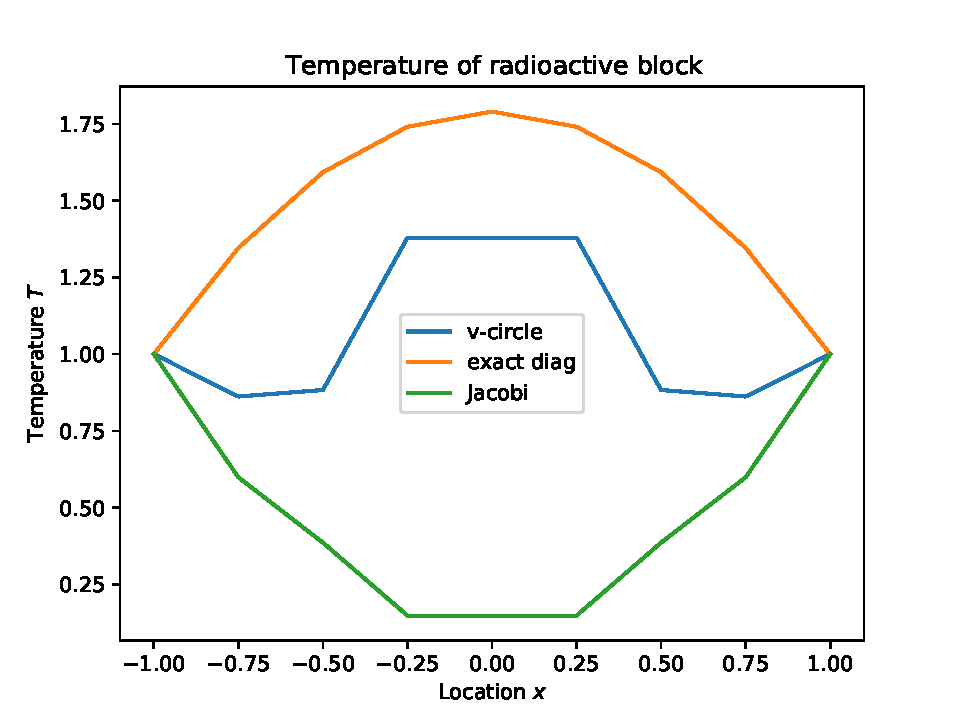
\includegraphics[width=.7\textwidth]{../figures/Aufg2e.pdf}
        % \caption{}
    \end{figure} \ \\ 
    The V-cycle method leads to a notable improvement compared to the 
    Jacobi method.
